\documentclass[12pt,a4paper]{article}
\usepackage[margin=1in]{geometry}
\usepackage{amsmath,amssymb,amsfonts}
\usepackage{graphicx}
\usepackage{float}
\usepackage{booktabs}
\usepackage{multirow}
\usepackage{array}
\usepackage{caption}
\usepackage{subcaption}
\usepackage{algorithm}
\usepackage{algorithmic}
\usepackage{url}
\usepackage[utf8]{inputenc}

\title{PinBallElsevier-2}
\author{Farzan Saeedi, Sanaz Keshvari, Hadi Sadoghi-Yazdi}
\date{}

\begin{document}
	
	\maketitle
	
	\begin{abstract}
		Predicting stock prices with the Kalman filter is a widely used model-based approach. A controllable Kalman filter is proposed to address some of the defects of the conventional Kalman filter by utilizing prior knowledge. Prior knowledge is derived from the history of data or related sources such as political, social, and economic conditions, sentiment analyses of news, indicators, and price action, or expert experience in the stock market. This approach has several advantages, one of which is reducing delay at sudden trend changes namely critical points. An algorithm is used to derive prior knowledge, which identifies resistance and support lines in stock prices.
		
		Controllable Kalman filters can be designed using a variety of approaches. Among these approaches, the use of controllable loss functions is a promising approach, with the PinBall loss function enabling the integration of prior knowledge into conventional Kalman filters. The PinBall loss function can be used to control Kalman filter parameters and addresses observation bias.
		
		An analysis and discussion of various types of stocks and synthesis stock was conducted theoretically. Compared with other methods like LSTM and ARIMA, the proposed method is more effective at evaluating the profit and loss functions of stock trades at critical points.
	\end{abstract}
	
	\section{Introduction}
	
	The stock market is a complex and dynamic system with noisy, non-stationary, and volatile data series. Thus, understanding the key drivers of stock market performance is critical for investors in order to make informed investment decisions. It has been attempted in recent years to detect sudden changes in volatility (1), however, it is challenging due to factors such as domestic, global, and political events, etc.(2).
	
	Various approaches to stock price prediction can be categorized as model-driven and data-driven. In the Model-driven category, Kalman filters were introduced with different loss functions, such as Mean Squared Error(MSE)(3), Correntropy (4), and Huber (5; 6). Data-driven models include Auto-Regression (AR) (7), Moving Average (MA) (8), and long-short-term memory (LSTM) (9). Existing stock price prediction models are dominated by formalization without considering prior knowledge, i.e., it is assumed that all stock price movement patterns follow the previous trend. Therefore, all points of stock price have the same impact on prediction, with the result that sudden changes have a delay in being predicted.
	
	There have been a number of model-driven methods developed in the past few years for predicting sudden changes in stock prices, including (10), (11), and (12). They add a new term to their model formulation besides the previous trend term. This supplementary term captures high changes in stock prices, which are not adequately captured by the existing trend term. These methods are able to identify high changes in stock prices and make more accurate predictions about future stock prices. By applying a different effect on trend change points, (10) added a seasonal term that assigns a periodic pattern to time series. The cycle term and periodic term defined by (11) and (12) are like a pulse that dampens the impact of stock price movement. Furthermore, these terms can help smooth out short-term volatility while offering additional insight into long-term trends. To manage non-periodic fluctuations (pulse) in the time series, they assumed other changes as noise which can be handled by regression of different time series and using spike and slab prior to initializing their iterative algorithm.
	
	Though a rich body of work deals with handling sudden changes in stock price prediction, very few studies have studied how to model the estimation of critical points using a Kalman filter model, which decreases the impact of previous points on prediction. The Kalman filter is designed to be able to adjust for any changes in inputs and to be able to respond quickly to new inputs. Therefore, when the Kalman filter detects a change that is out of the ordinary, it can indicate that there is an unknown input that is causing the change (13). The uncertainty problem in non-linear time series is solved by estimating weights for the modeling loss function by adding various effects of observation in (14). (15) modeling exciting changes in time series, which cause a drift in estimated input, by dual Kalman filter.
	
	This paper addresses this problem by introducing a modified Kalman filter that has prior knowledge and reduces the delay in sudden changes in stock price prediction while maintaining convergence. Here, the main intuition is that there are different impacts on the estimation and prediction of model state space. As a prior knowledge, an algorithm extracts sudden changes from observations in the proposed Kalman filter model. Additionally, the Kalman filter model incorporates Pinball loss functions to modify prediction delays. The proposed Kalman filter uses the Pinball loss function to modify prediction delay by defining prior knowledge in order to extract sudden changes from observation by the proposed algorithm.
	
	Using the Kalman filter, prior knowledge is incorporated into the Kalman gain step and the Kalman prediction step is then used to develop KF-Pinball, a novel stock price prediction model. By adding Pinball to the Kalman filter, two models are defined: KF-SGD-PinBall and KF-PseudoPinball. Based on the theoretical analysis of the Kalman filter, we show the profitability of the following stock when a sudden change in stock price occurs. A flowchart illustrating how to add prior to the Kalman filter model is shown in Figure 1. According to this figure, prior knowledge influences both the loss function and the state space prediction.
	
	An evaluation of the proposed stock price prediction algorithm is conducted on Yahoo Finance stock. These stocks are selected based on close prices from 01.01.2020 to 01.01.2021. Using a variety of evaluation metrics, we show that the modified Kalman filter model outperforms the Data-driven and Model-driven models.
	
	In summary, the paper's major contribution is as follows:
	\begin{itemize}
		\item The Kalman filter is modified to incorporate prior knowledge of observation.
		\item The state space in this Kalman filter is updated with different effects at critical points.
		\item The behavior of the proposed Kalman filter with Pinball loss function is theoretically discussed and analyzed, i.e. whether the adjustment of pinball loss is consistent with stock price movements.
		\item The proposed Kalman filter is empirically evaluated with Data-driven and Model-driven methods on the Yahoo Finance dataset in the area of profit performance at critical points.
	\end{itemize}
	
	As shown in the following outline, this paper is organized as follows: The next section discusses related work on stock price prediction and Kalman filter characteristics. A Kalman filter pseudo Pinball and Kalman SGD Pinball model are introduced in Section 3. To evaluate the proposed learning model, we conducted a comprehensive set of experiments in Section 4. Lastly, Section 5 concludes the paper.
	
	\section{Related works}
	
	The stock marketing challenge can be categorized into a variety of categories, such as prediction and decisionmaking. The decision-making process for the stock price is carried out using both technical analysis (E.g. moving average convergence/divergence (MACD) (16)) and fundamental analysis (E.g. news analysis). There are two methods for predicting stock prices, statistical methods and machine learning methods (17). Statistical methods are such as Auto-Regressive (AR) (7), Moving Average (MA) (7), and Kalman filter. Also, machine learning methods are like decision tree (DT) (18), Random forest (RF)(18), and long-short-term memory (LSTM) (9). This paper focuses on statistical methods for stock price prediction.
	
	Since of satisfied model does not exist for the stock price makes it is difficult to predict stock prices using statistical methods. Machine learning methods make better estimates by monitoring observations over time. Due to the lack of a definite pattern for some time series, such as the stock market, machine learning cannot be used effectively.
	
	Statistical methods for stock price prediction begin with a based model like AR and MA. The AR model utilizes a weighted summation of previous observations with noise to predict future observations. The MA model calculates the summation of a parameter with Gaussian noises which are assumed to have the same variance. The next two methods are the Auto-Regressive Moving Average (ARMA) and the Auto-Regressive Integrated Moving Average (ARIMA), which combines the AR and MA methods where observational information is provided by AR, and noise information is provided by MA. ARIMA is an efficient method for nonstationary time series like stock prices since it combines ARMA with the finite derivative of previous observations (7).
	
	Several studies have shown that Kalman filters are better than complex LSTM at low volatility stock predicting (19). A Kalman filter has been shown to be better than machine learning methods in COVID-19 because of abnormal fluctuations in the price of digital currencies (20). It is because, in this situation, the Kalman filter follows the model instead of previous observations. In order to address the unsolved challenge of Kalman filters with regard to the identification and reversal of critical points, we use PinBall loss functions.
	
	Pinball loss functions have been used for different types of machine-learning problems like classification (21) and clustering (22) in recent years. By using this asymmetric function, noise-insensitive versions of support vector machines can be derived.
	
	\subsection{Kalman filter}
	
	Most of the time series have been processed with the Kalman filter (23; 24; 25). This uses the Bayesian rule in orthogonal principle (26) and assumes Gaussian noise for the input and model, and it predicts the next data, based on the statistical model and the current data. By minimizing the covariance of the difference between ground truth and estimation of state space, this method smooths observation and computational noise. In Eq. 1, \(Y\) represents observations with \(n \times 1\) dimensions; \(X\) illustrates model parameters with \(n \times d\) dimensions; The index \(t\) represents parameter values in time \(t\). Using \(\sim\) and \(\Lambda\) to estimate parameters (in update phase) and predict parameters.
	
	\begin{equation}
		\begin{array}{rl} 
			& y_t = Hx_t + \epsilon_t,\qquad \epsilon_t\sim N(0,R)\\
			& x_t = Fx_{t - 1} + Z\eta_t,\qquad \eta_t\sim N(0,Q) 
		\end{array} \quad (1)
	\end{equation}
	
	The Kalman filter follows these steps:
	
	\begin{equation}
		\begin{array}{rl} 
			& 1.\left\{ \begin{array}{ll}\hat{y}_t = H\hat{x}_{t - 1},\\
				\hat{x}_t = F\hat{x}_{t - 1} + Bu_{t - 1} \end{array} \right.\\
			& 2.\hat{P}_t = F\hat{P}_{t - 1}F^T + ZQZ^T,\\
			& 3.K_t = \hat{P}_tH^T (H\hat{P}_tH^T +R)^{- 1},\\
			& 4.\hat{x}_t = \hat{x}_t + K_t(y_t - H\hat{x}_t),\\
			& 5.\hat{P}_t = (I - K_tH)\hat{P}_t(I - K_tH)^T +K_tRK_t^T 
		\end{array} \quad (2)
	\end{equation}
	
	These equations are based on the notation that \(F\) is a \(d \times d\) state space transition matrix, \(H\) is a \(1 \times d\) observation transition matrix, \(R\) is observation variance, \(Q\) is a \(q \times q\) computational covariance matrix, \(B\) is a \(d \times b\) control matrix for input, \(u_t\) is a \(b \times 1\) input vector, \(P\) is \(d \times d\) state space error covariance parameters and \(Z\) in a \(d \times q\) is a mapping matrix that maps computational noise covariance to state space error covariance.
	
	Eq. 2 demonstrated the MSE loss function applied to the Kalman filter by default (orthogonal principle). When the loss function is changed, the Kalman gain (step 3 in Eq. 2) also changes. This step adjusts the estimate parameters (steps 4 and 5 in Eq. 2). The CorrEntropy loss function (4) reformulated the gain step by using Weighted Least Square (WLS) (27) method in the formulation as follows:
	
	\begin{equation}
		\begin{array}{rl} 
			& K_t = \frac{C_tH^T R^{-1}}{\hat{P}_t^{-1} + C_tH^T R^{-1}H},\\
			& C_t = \frac{G_\sigma(\|y_t - H\hat{x}_t\|_{R^{-1}}^2)}{G_\sigma(\|x_t - F\hat{x}_{t - 1}\|_{P_t^{-1}}^2)},\\
			& G_\sigma (x) = 1 - \exp (\frac{-x}{2\sigma^2}),\quad x\geq 0 
		\end{array} \quad (3)
	\end{equation}
	
	When MSE and CorrEntropy loss functions are used, both have a delay at a critical point. To examine delay at critical points, the Huber loss function was applied (5; 6) then due to the non-continuous derivation of this function, we used a Pseudo-Huber loss function (28) without further analysis and reformulate Kalman filter's gain as follows:
	
	\begin{equation}
		\begin{array}{rl} 
			& K_t = \frac{C_tH^T R^{-1}}{\hat{P}_t^{-1} + C_tH^T R^{-1}H},\\
			& C_t = \frac{\sqrt{1 + (\|x_t - F\hat{x}_{t - 1}\|_{P_t^{-1}}^2 / \delta)^2}}{\sqrt{1 + (\|y_t - H\hat{x}_t\|_{R^{-1}}^2 / \delta)^2}} 
		\end{array} \quad (4)
	\end{equation}
	
	Fig. 2 shows the estimation of observations using different loss functions. Identification of critical points and reversal of critical points are delayed by all three methods. It is necessary to have prior knowledge about the critical point in order to identify it. The ability of different loss functions to reverse at critical points is various since different Kalman gain functions adjust the parameters differently. It is important to note that the MSE and Pseudo-Huber loss functions have more delay on reversal of critical points than the corrEntropy loss function, as they are sensitive to outlier data, while the corrEntropy loss function is insensitive to outlier data.
	
	Loss functions are compared by using different parameters in Fig. 6, (e.g., \(\sigma\) in the corrEntropy loss function in equation Eq. 3 and \(\delta\) in the Pseudo-Huber loss function in equation Eq. 4). Note that the majority of \(\sigma\) have the same results, so figure Fig. 6 shows two instances but does not show others. Additionally, various values of \(\delta\) in the Pseudo-Huber loss function are selected to give the best results for the range [0.25-3].
	
	\begin{figure}[H]
		\centering
		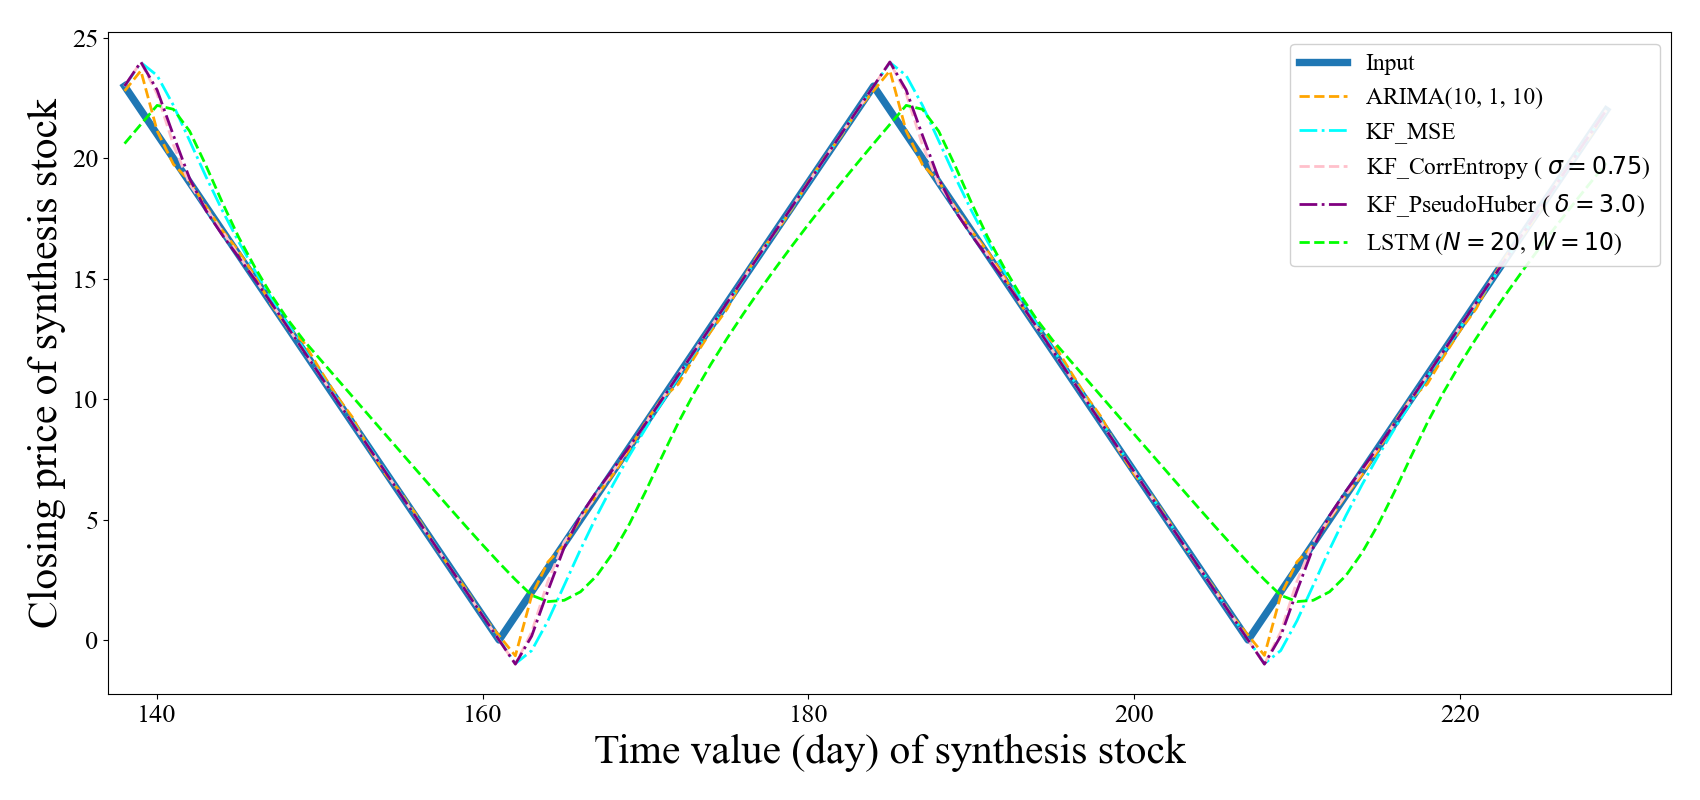
\includegraphics[width=0.8\textwidth]{figure2.png}
		\caption{The blue line shows synthesized time series that are predicted by ARIMA, LSTM as data-driven models, and Kalman Filter Mean Squared loss function (KF MSE), Kalman Filter Corr Entropy loss function (KF CorrEntropy) and Kalman Filter pseudo-Huber (KF pseudoHuber) as model-driven models. The critical points in all of them are predicted with delays at their peaks and valleys.}
		\label{fig:figure2}
	\end{figure}
	
	\begin{figure}[H]
		\centering
		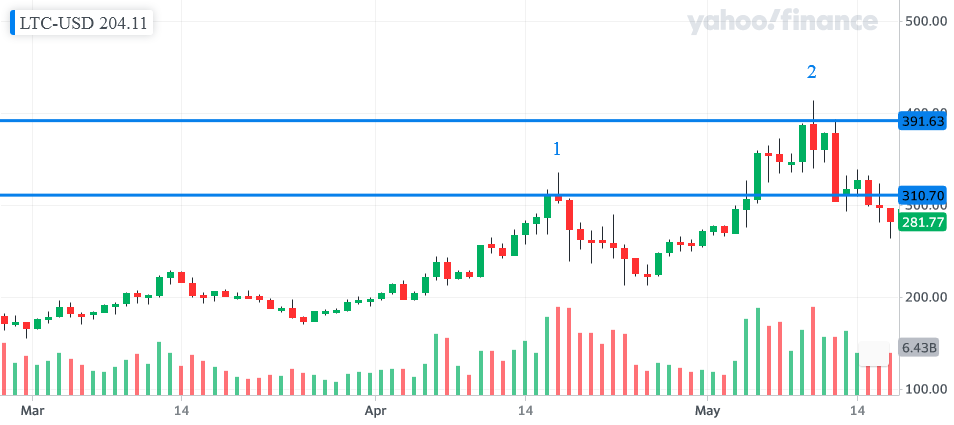
\includegraphics[width=0.8\textwidth]{figure3.png}
		\caption{LTC's critical point in the part of a daily timeframe of 2021. Points 1 and 2 show the peak of LTC.}
		\label{fig:figure3}
	\end{figure}
	
	\begin{figure}[H]
		\centering
		\begin{subfigure}{0.48\textwidth}
			\centering
			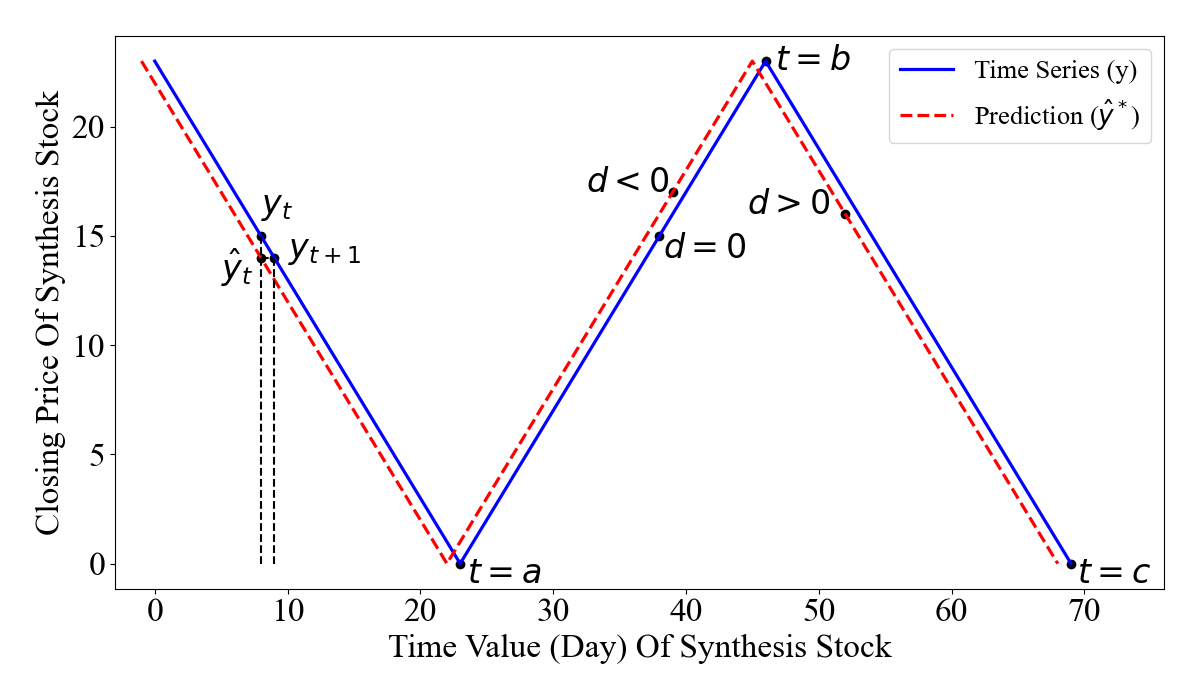
\includegraphics[width=\textwidth]{figure4a.png}
			\caption{The blue line represents the synthesis stock, and the red dashed line is the most accurate stock prediction.}
		\end{subfigure}
		\hfill
		\begin{subfigure}{0.48\textwidth}
			\centering
			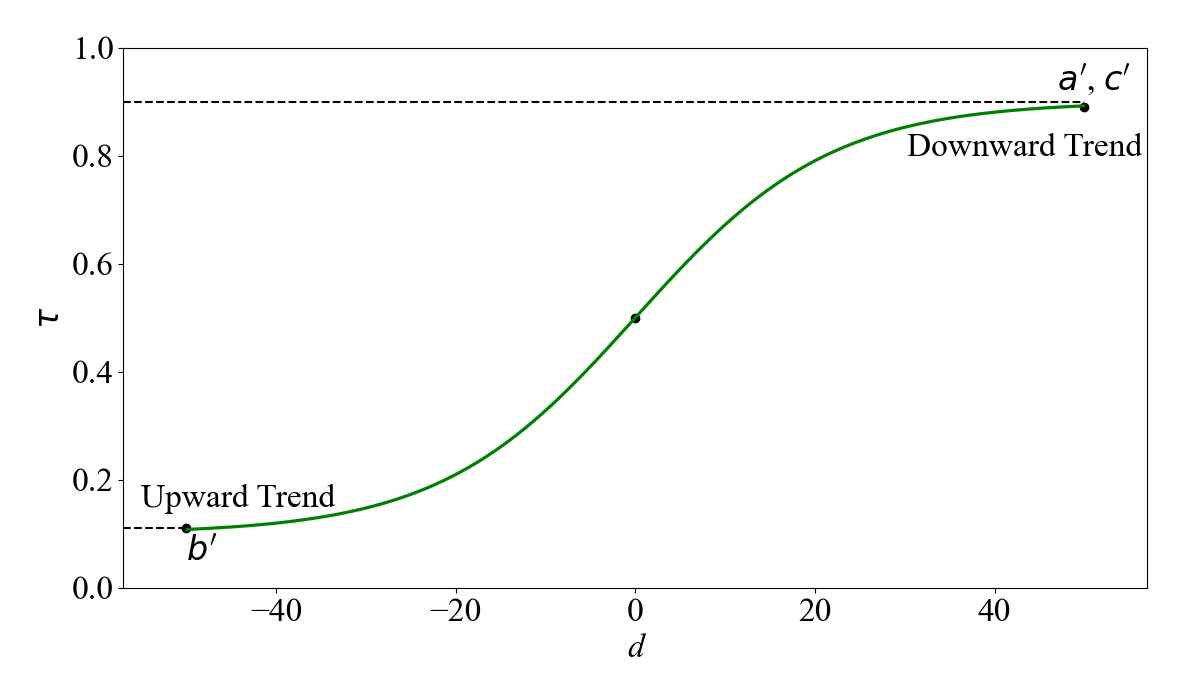
\includegraphics[width=\textwidth]{figure4b.png}
			\caption{\(\tau\) change per \(d\), where \(d = y-\hat{y}\).}
		\end{subfigure}
		\caption{Analyse of \(\tau\) parameter in the Pinball loss function. Adjusting \(\tau\) parameters of the Pinball loss function is essential to leverage prior knowledge of the Kalman filter. The upward trend in (a) (point \(a\) to point \(b\)) the \(\tau\) change from point \(d^{\prime}\) to point \(b^{\prime}\) in (b). The downward trend in (a) (point \(b\) to point \(c\)) the \(\tau\) change from point \(b^{\prime}\) to point \(c^{\prime}\) in (b).}
		\label{fig:figure4}
	\end{figure}
	
	The solution to obviate the delay of critical points consists of resolving two problems: 1. Identification of critical points, 2. Reversing movement trends rapidly on critical points for more precise parameter adjustments. In order to solve the first problem, we add prior knowledge to the Kalman filter model. Our solution to the second problem is using a Pinball loss function that can rapidly revert movement trends on critical points.
	
	\section{Proposed Method}
	
	\subsection{Motivation Example}
	
	Fig. 3 illustrates itecoin (LTC)'s critical points in the 2021 daily timeframe. The peaks of LTC in this timeframe can be seen at points 1 and 2. Model-driven approaches are not able to predict these points since there is no specific mathematical model for them, so it is impossible to assume one. Data-driven approaches have a delay in predicting critical points as well since these points have no identifiable pattern. It is still possible to calculate these support and resistance points from some kind of indicator and use them to predict stock prices. In order to reduce the delay between critical points in stock price prediction, we are motivated to add support and resistance lines as prior knowledge to the Kalman filter model.
	
	In order to create a Kalman filter model, the statistical model and the data must work together. If just data is used to estimate the stock price with the Kalman filter, the estimation of critical points has a delay. However, if a specific model is used, the estimation can be improved. Thus, we propose Kalman filter estimation of stock price by employing an appropriate model. Model parameters are adjusted based on the loss function. Due to delay reduction, the Pinball loss is introduced that is flexible for different errors, which enables more accurate model parameter adjustment and less delay.
	
	\subsection{Prior Knowledge}
	
	The term prior knowledge refers to knowledge that is derived from the history of data or related data sources. When the model does not follow the pattern of data, this knowledge can be used to outperform it. Also, it can leverage knowledge to model without processing all the history of data.
	
	Different types of prior knowledge are used depending on the problem. The conventional Kalman filter works by taking prior knowledge of the system on points that have estimation or prediction defects. This knowledge is combined with the current data from the system to make better predictions and make more accurate predictions about the system's behavior. As shown in Fig. 5, There are several types of prior knowledge in stock price prediction, including political, social, and economic conditions in (29), sentiment analysis of news on social media (e.g. Twitter, CNN, Etc.) in (30), indicators, price actions, or expert experiences can all be added to the Kalman filter to make it more accurate.
	
	In this work, prior knowledge is used to detect sudden change points to control the model at those points and make better estimations or predictions.
	
	\begin{figure}[H]
		\centering
		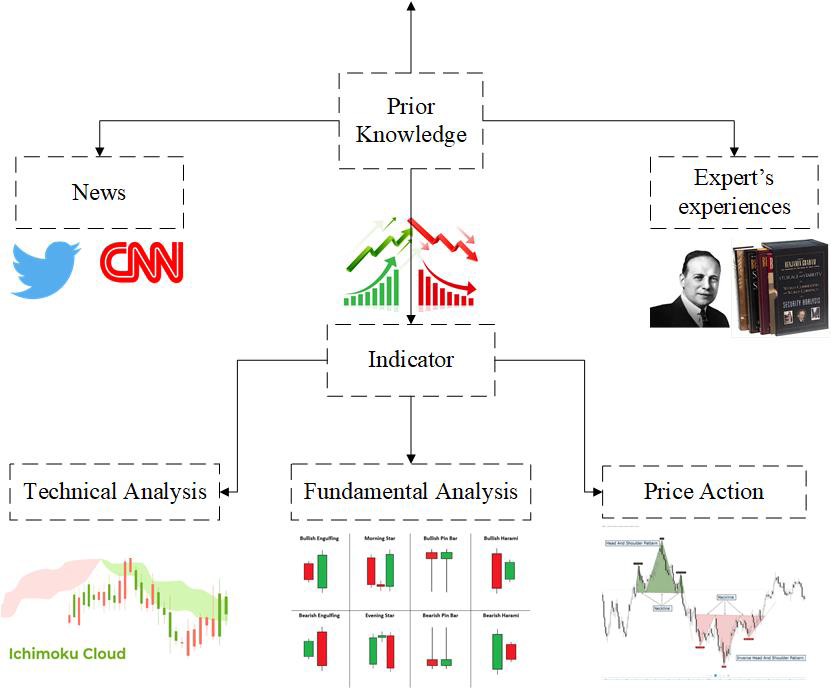
\includegraphics[width=0.8\textwidth]{figure5.png}
		\caption{The various kind of prior knowledge in stock price.}
		\label{fig:figure5}
	\end{figure}
	
	\subsection{Controllable Kalman Filter}
	
	As a consequence of reducing delay on critical points as a challenge, we reformulate the Kalman filter with the Pinball loss function.
	
	Pinball loss is a piecewise function Eq. 5; this causes the function to be asymmetric, and it gives different losses to positive and negative errors of estimation according to a flexible parameter \((\tau)\) which can address the challenge of reversing critical points. The ability to change in face of different errors based on prior knowledge is also beneficial.
	
	\begin{equation}
		L_{\tau}(y,\hat{y}) = \left\{ \begin{array}{ll}(y - \hat{y})\tau & y\geq \hat{y}\\ (\hat{y} - y)(1 - \tau) & \hat{y}\geq y \end{array} \right.,0< \tau < 1 \quad (5)
	\end{equation}
	
	Adding the Pinball loss function to the Kalman filter, based on WLS, requires derivation of the function, and the Pinball loss function has not had continuous derivation when observation is zero. To address this issue, we propose two approaches: Pseudo-Pinball and Kalman gradient descent by the Pinball loss function.
	
	According to Fig. 4, the flexible parameter \((\tau)\) is explained as follows. There are different types of loss functions shown in Fig. 6, all of them except the Pinball loss function are symmetric functions, and the reason for this is the \(\tau\) parameter in formulation Eq. 5 (e.g in the Pinball loss function \(f(2) \neq f(- 2) \tau \neq 0.5)\). \(\tau\) is used to adjust the derivation of the line in the first and second regions of the coordinates in the Pinball loss function. Prior knowledge can always be used to adjust this parameter to get the most accurate time series prediction. To understand how \(\tau\) changes, we need to analyze the most accurate prediction of the time series in Fig. 4a. As shown in Fig. 4a, the most accurate prediction of \(y\) (blue line) is \(\hat{y}^{*}\) (red dashed line). At time \(t\), the time series value is \(y_{t}\), the most accurate prediction intends \(y_{t + 1}\); therefore, the most accurate prediction of \(y_{t}\) is \(\hat{y}_{t}^{*}\), since \(\hat{y}_{t}^{*} = y_{t + 1}\).
	
	Taking \(d = y - \hat{y}\) as shown in Fig. 4a, \(d < 0\) in an upward trend when \(\hat{y} > y\) and \(d > 0\) in a downward trend when \(\hat{y} < y\). Based on Fig. 4a let \(t = a\) indicate the endpoint of a downward trend and a beginning point of an upward trend, then based on the Fig. 4b, \(d^{\prime}\) is the similar point of \(a\), in this point \(\tau\) parameter of Pinball loss is 0.9. Moving from point \(a\) to point \(b\) will give the most accurate prediction in an upward trend \((d < 0)\) in Fig. 4a, during this move, \(\tau\) values must steadily decrease to \(\tau = 0.1\) in Fig. 4b. In contrast, downward trend \((d > 0)\), \(\tau\) values must steadily increase (by moving from \(b\) to \(c\) in Fig. 4a at similar points \(b^{\prime}\) to \(c^{\prime}\) in Fig. 4b).
	
	\begin{figure}[H]
		\centering
		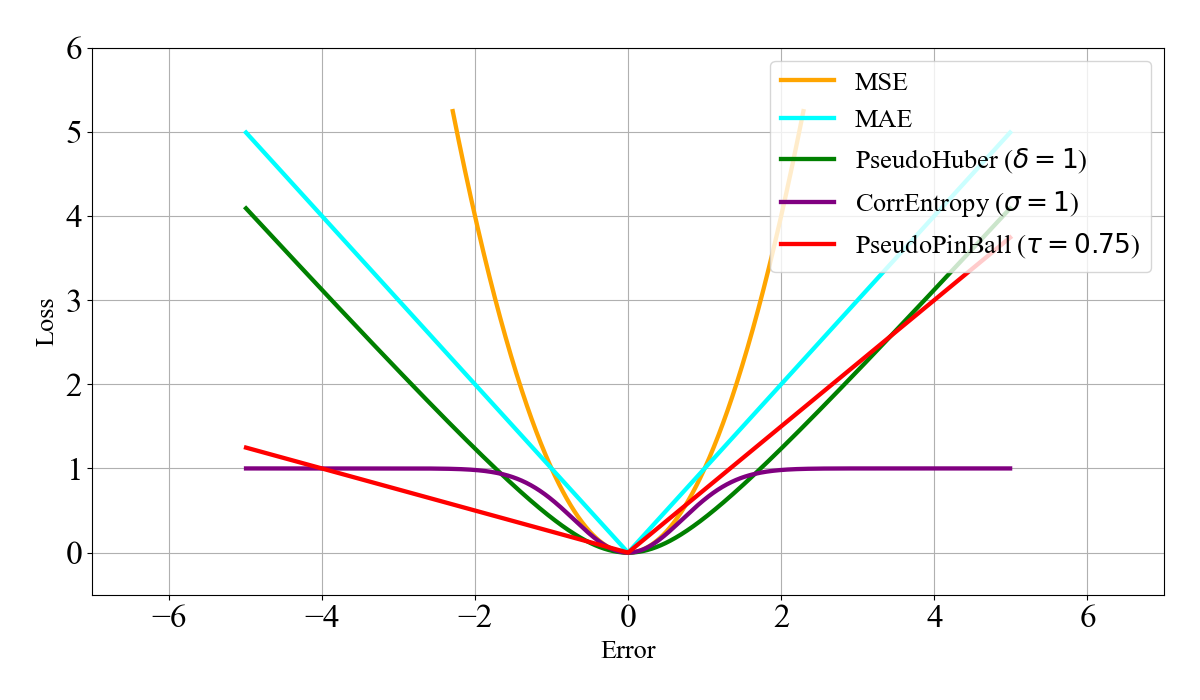
\includegraphics[width=0.8\textwidth]{figure6.png}
		\caption{Asymmetric pinball loss functions and various symmetric loss functions.}
		\label{fig:figure6}
	\end{figure}
	
	\subsubsection{The Proposed Pseudo-Pinball loss function}
	
	Reconstruct the pinball loss function by using two tanh functions Eq. 6; this simulation is called Pseudo-Pinball.
	
	\begin{equation}
		\begin{array}{l}{L = (\tau)e^{\frac{\tanh(4e) + 1}{2}} + (\tau -1)e^{\frac{\tanh(4e) + 1}{2}}}\\
			{= \frac{(2\tau - 1)e\tanh(-4e)}{2}} 
		\end{array} \quad (6)
	\end{equation}
	
	Calculate the minimum error when derivation of Eq. 6 equals zero and it rewrites the Kalman gain function as Eq. 7.
	
	\begin{equation}
		\begin{array}{l}{K_{t} = \frac{C_{t}H^{T}R^{-1}}{\hat{P}_{t}^{-1} + C_{t}H^{T}R^{-1}H},}\\
			{C_{t} = \frac{G_{\tau}(\|y_{t} - H\bar{x}_{t}\|_{R^{-1}})}{G_{\tau}(\|x_{t} - F\bar{x}_{t - 1}\|_{P_{t}^{-1}})},}\\
			{G_{\tau}(x) = \frac{\sinh 8x + 8x}{\cosh 8x + 1} -(1 - 2\tau),x\geq 0} 
		\end{array} \quad (7)
	\end{equation}
	
	The prior knowledge is derived from two steps: smoothing by the moving average and finding critical points. A moving average method with fixed weights is used in which its window is a vector \(1 \times w\), and the elements are \(\frac{1}{w}\) that is convoluted with the equivalent observation window. We then use Algorithm. 1 to find critical points, Its input is the output of the convolution step, and the output is critical points. Kalman filter can be applied with prior knowledge by using the Pinball loss function. Due to having a flexible parameter, adding prior knowledge is easily possible.
	
	\begin{algorithm}
		\caption{Find Peaks}
		\begin{algorithmic}[1]
			\STATE Data: Time Series, Critical Point Distance, Prominence Length
			\STATE Result: Peaks Indices
			\STATE Peaks \(= []\)
			\FOR{i in range (length of Time Series)}
			\IF{(Time Series[i] \(\geq\) Time Series[i - 1] and Time Series[i] \(\geq\) Time Series[i + 1] and i - Peaks[-1] \(\geq\) Critical Point Distance)}
			\STATE Selected Peak \(= 1\)
			\FOR{j in Time Series [i - Prominence Length: i + Prominence Length]}
			\IF{$i \neq j$ \& Time Series[j] \(\geq\) Time Series[i]}
			\STATE Selected Peak \(= 0\)
			\ENDIF
			\ENDFOR
			\IF{Selected Peak \(== 1\)}
			\STATE Append i to Peaks
			\ENDIF
			\ENDIF
			\ENDFOR
		\end{algorithmic}
	\end{algorithm}
	
	\subsubsection{Stochastic Gradient Descent (SGD) Pinball loss function}
	
	The second way to deal with the pinball loss function's non-differentiable nature is to use a SGD formulation instead of a Kalman filter formulation. As an alternative to updating Kalman filter estimation parameters, this approach is used from formulation 8.
	
	\begin{equation}
		\begin{array}{rl} 
			& 1.\left\{ \begin{array}{ll}\hat{y}_t = H\hat{x}_{t - 1},\\
				\hat{x}_t = F\hat{x}_{t - 1} \end{array} \right.\\
			& 2.\hat{P}_t = F\hat{P}_{t - 1}F^T +ZQZ^T,\\
			& 3.\left\{ \begin{array}{ll}J = H^TL(\| y_t - H\hat{x}_t\|_{R - 1}) + L(\| \hat{x}_t - F\hat{x}_{t - 1}\|_{\hat{P}_t^{- 1}}),\\
				\hat{x}_t = \hat{x}_t - \mu \frac{\partial J}{\partial\hat{x}_t} \end{array} \right.\\
			& 4.\hat{P}_t = E\{\hat{x}_t^T\hat{x}_t\} 
		\end{array} \quad (8)
	\end{equation}
	
	where \(\mu\) is the learning rate which needs to be determined by the expert or calculated empirically, \(J\) is the cost function and \(L\) is the Pinball loss function; As an alternative to updating Kalman filter estimation parameters (step 3 of formula Eq. 2), this approach is used \(- \mu \frac{\partial J}{\partial\hat{x}_t}\) (step 3 of formula Eq. 8). With the Kalman filter, we calculate the prediction error \((y_t - H\hat{x}_t)\) and multiply by \(K_t\) to adjust the parameters. In this method, the parameters are adjusted by minimizing prediction error and learning rate. An essential aspect of this algorithm is defining the learning rate.
	
	\subsection{Derived Controllable Kalman Filter Using Bayesian Filter}
	
	A Bayesian optimal filtering approach was used by (31). to derive the Kalman filter. Here we prove that controllable Kalman filters can be derived as Bayesian optimal filters, similar to simple Kalman filters. As mentioned before, Kalman filters are based on the Bayesian theorem, with the probability of the normal distribution being represented by Eq. 9. We add prior knowledge to a simple Kalman filter to control prediction at critical points. Here, we want to show that the controllable Kalman filter has a normal distribution probability after adding prior knowledge. So, it can be derived as a Bayesian optimal filter like (31). The Eq. 9 is the Bayesian theorem in Kalman filter form. This equation consists of \(p(y_t|x_t)\) which is the prediction of observation according to state space prediction in time \(t\), \(p(x_t|y_{0:t - 1})\) is the prediction of state space in time \(t\), and \(p(y_t|y_{0:t - 1})\) is the observation in time \(t\).
	
	\begin{equation}
		p(x_t|y_{0:t}) = \frac{p(y_t|x_t)p(x_t|y_{0:t - 1})}{p(y_t|y_{0:t - 1})} \quad (9)
	\end{equation}
	
	Based on independent and identically distributed (IID) variables, \(E\{\epsilon_t|y_{0:t - 1}\} = E\{\eta_{t - 1}|y_{0:t - 1}\} = E\{u_{t - 1}|y_{0:t - 1}\} = 0\). Adding the prior knowledge to the Kalman filter affects the prediction steps because the prior knowledge is incorporated into the prediction of the state vector and the error covariance matrix (steps 1 and 2 of Eq. 2). The right-hand side of Eq. 9 is calculated after the prior knowledge is added in Eq. 10 because it depends on the prediction of the state vector and the error covariance matrix.
	
	\begin{equation}
		\left\{ \begin{array}{ll}E\{y_t|x_t\} & = E\{Hx_t + \epsilon_t|x_t\} = Hx_t,\\
			var(y_t|x_t) & = E\{y_t,y_t^T|x_t\} = R\\
			& \Rightarrow p(y_t|x_t) = N(y_t|Hx_t,R) \end{array} \right.
	\end{equation}
	
	\begin{equation}
		\left\{ \begin{array}{ll}E\{x_t|y_{0:t - 1}\} & = E\{F\hat{x}_{t - 1} + Bu_{t - 1} + Z\eta_{t - 1}|y_{0:t - 1}\} \\
			& = F\hat{x}_{t - 1} = \hat{x}_t,\\
			cov(x_t|y_{0:t - 1}) & = E\{x_t,x_t^T|y_{0:t - 1}\} \\
			& = F\{E\{\hat{x}_{t - 1}\hat{x}_{t - 1}^T|y_{0:t - 1}\} F^T \\
			& +BE\{\hat{u}_{t - 1}\hat{u}_{t - 1}^T|y_{0:t - 1}\} B^T \\
			& +ZE\{\hat{\eta}_{t - 1}\hat{\eta}_{t - 1}^T|y_{0:t - 1}\} Z^T = \hat{P}_t \end{array} \right.
	\end{equation}
	
	\begin{equation}
		\left\{ \begin{array}{ll}E\{y_t|y_{0:t - 1}\} & = E\{H(F\hat{x}_{t - 1} + Bu_{t - 1} + Z\eta_{t - 1})\\
			& +e_t|y_{0:t - 1}\} = H\hat{x}_t,\\
			var(y_t|y_{0:t - 1}) & = E\{y_t,y_t^T|y_{0:t - 1}\} \\
			& = HE\{x_t,x_t^T|y_{0:t - 1}\} H^T +R\\
			& = H\hat{P}_tH^T +R\\
			& \Rightarrow p(y_t|y_{0:t - 1}) = N(y_t|H\hat{x}_t,H\hat{P}_tH^T +R) \end{array} \right. \quad (10)
	\end{equation}
	
	where \(E\{.\}\) is expectation operation, var(.) is the variance, and cov(.) is covariance that derived from the Kalman filter steps. due to assuming each density as a normal distribution, \(E\{.\}\),var(.),and cov(.) expanded.
	
	It is obvious that the production of normal densities will be a normal density with mixed mean and variance from the other distributions. There are two approaches to defining prior knowledge for this research usage. First, assume it happens at a special time (like the first day of a month). The second approach is to assume prior knowledge as a time series whose values range between 0 and 1, as a probability of trend reversal. In both approaches, the variance of prior knowledge is less than 1, so the Kalman filter prediction is low. In this research, the first approach is used.
	
	The covariance of prediction (known as \(\hat{p}\)) indicates how much variance is acceptable for prediction. The prior knowledge covariance term \(\left(BE\{\tilde{u}_{t - 1}\tilde{u}_{t - 1}^T |y_{0:t - 1}\} B^T\right)\) allows for more variance in the prediction, which means that the prediction can deviate more from the previous state. This is important for trend reversals, as the prediction needs to be able to break away from the previous trend in order to accurately predict the new trend. As well, it affects estimation by not updating recent predictions for following previous trends on reversal points.
	
	\section{Experimental}
	
	\subsection{Research objectives}
	
	This section evaluates the performance of the Kalman filter using the PinBall loss function. Two research objectives are examined through our experiments:
	
	Research Objective 1: Stock Price Prediction Performance We evaluate our proposed method using synthetic data and stocks in Tables. 1. The stocks were all selected for the daily time-frames between 2020.01.01 and 2021.01.01. Research Objective 2: Profitability and error analysis In order to evaluate the effectiveness of our tradebased methods, two evaluation measurements are carried out: first, the loss function, and second, the profit from trades using synthetic data and CSCO stock.
	
	\subsection{Dataset}
	
	The proposed method is evaluated and compared with other methods using synthesis data and existing stocks in this section of the experiment. The Stocks are in the yahoo finance. Tesla Inc, Apple Inc, Cisco Systems Inc, Amazon.com Inc, Advanced Micro Devices Inc, Carnival Corporation \& plc, NVIDIA Corporation, Futu Holding Limited, iQIYI Inc, Alphabet Inc(formerly known as Google, with and without voting), The Walt Disney Company, Shopify Inc, Micron Technology Inc, Alibaba Group Holding Limited, Exxon Mobil Corporation, Norwegian Cruise Line Holdings Ltd, Citigroup Inc, Intel Corporation, Microsoft Corporation, and DraftKings Inc from 2020.01.01 to 2021.01.01 are used.
	
	We compute prior knowledge by applying Algorithm. 1 to all stocks, which means support and resistance lines. This leverages prior knowledge of critical points in the Kalman filter by adjusting the \(\tau\) parameter of the PinBall loss function. The aim of the Kalman filter with Pinball loss function is to reduce the delay in identifying critical points and reversing them, to evaluate this aim a profit measure defines in the Experimental setup section and the result of this measure is reported in the Experimental result section.
	
	\begin{figure}[H]
		\centering
		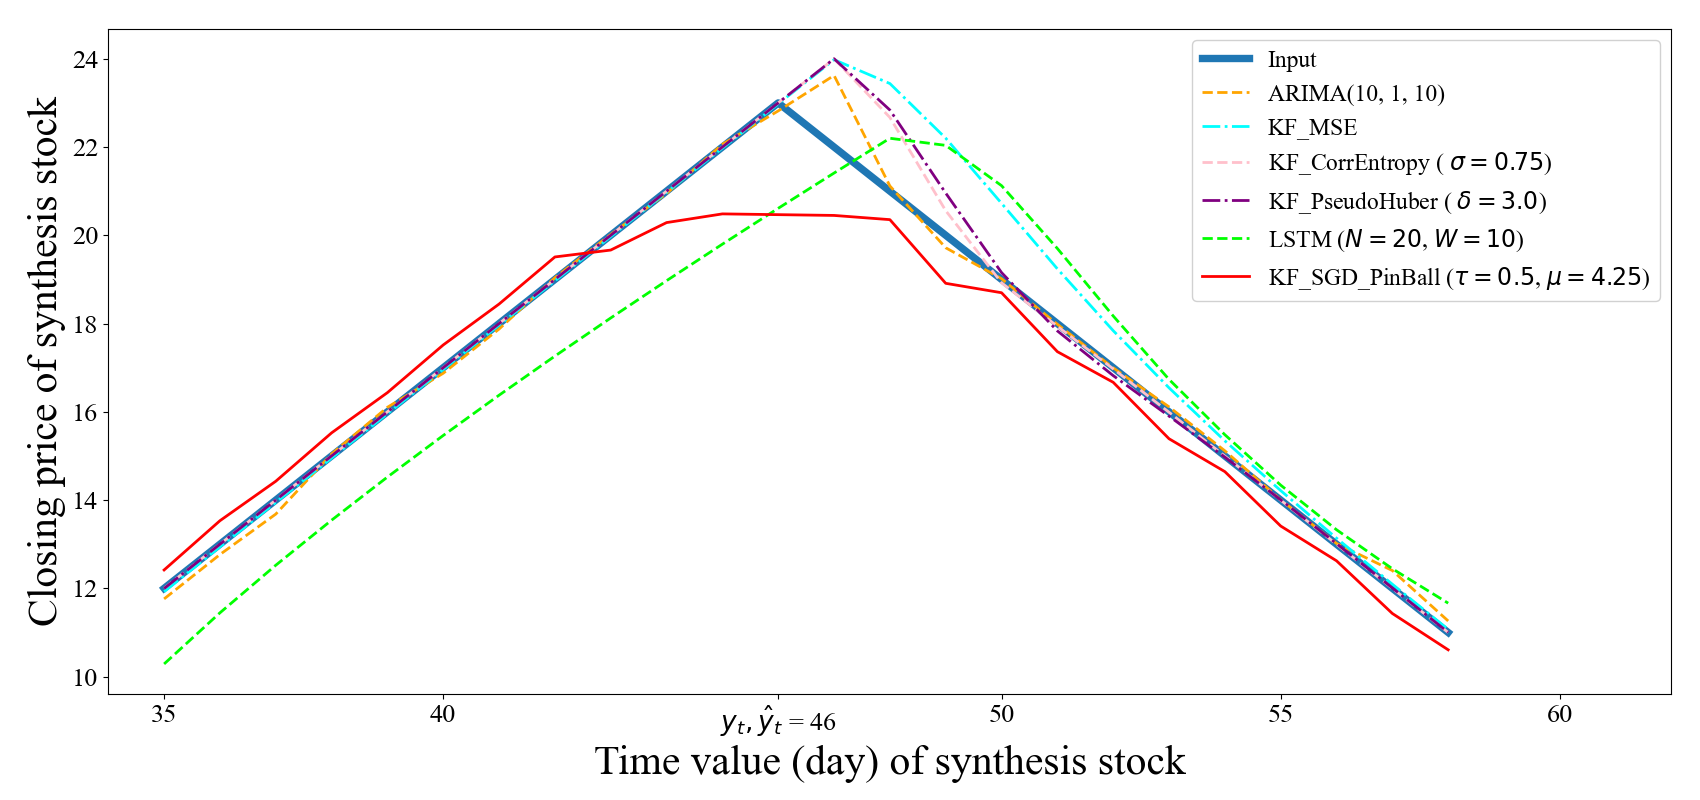
\includegraphics[width=0.8\textwidth]{figure7.png}
		\caption{Predictions of peak profits in the synthesis stock. \(y_{t} = 46\) corresponds to the synthesis stock peak. \(\hat{y}_{t}\) represents the prediction of the synthesis stock by prediction methods that is shifted one step forward.}
		\label{fig:figure7}
	\end{figure}
	
	\begin{table}[H]
		\centering
		\caption{Stock symbols}
		\begin{tabular}{ll}
			\hline
			\textbf{Stock Name} & \textbf{Symbol} \\
			\hline
			Tesla Inc & TSLA \\
			Apple Inc & AAPL \\
			Cisco Systems Inc & CSCO \\
			Amazon.com Inc & AMZN \\
			Advanced Micro Devices Inc & AMD \\
			Carnival Corporation \& plc & CCL \\
			NVIDIA Corporation & NVDA \\
			Futu Holding Limited & FUTU \\
			iQIYI Inc & IQ \\
			Alphabet Inc (with voting) & GOOGL \\
			The Walt Disney Company & DIS \\
			Shopify Inc & SHOP \\
			Micron Technology Inc & MU \\
			Alibaba Group Holding Limited & BABA \\
			Exxon Mobil Corporation & XOM \\
			Norwegian Cruise Line Holdings Ltd & NCLH \\
			Citigroup Inc & C \\
			Intel Corporation & INTC \\
			Alphabet Inc (without voting) & GOOG \\
			Microsoft Corporation & MSFT \\
			DraftKings Inc & DKNG \\
			\hline
		\end{tabular}
		\label{tab:table1}
	\end{table}
	
	\subsection{Experimental setup}
	
	Implementation of the proposed and other methods is carried out using Python, and loss functions are calculated using the formulations provided in previous sections. The CorrEntropy loss function has a parameter \(\sigma\) and the Pseudo Hubber loss function has a parameter \(\delta\) we implement these models in a range and then report the lowest loss result in the experimental result.

	The Python scripts used for generating the experimental comparisons, plots, tables, and statistical tests are included with this manuscript in the \texttt{code\_PinBall\_Kalman} folder.
	
	\subsection{Result}
	
	\subsubsection{Research objective 1: Stock price prediction performance}
	
	In this section, the stock profit performance of the proposed methods named KF Pseudo-Pinball and KF SGD Pinball will be evaluated and compared with data-driven methods and model-driven methods on TSLA, AAPL, AMZN, AMD, CCL, NVDA, FUTU, IQ, GOOGL, DIS, SHOP, MU, BABA, XOM, NCLH, C, INTC, MSFT, and DKNG. We use profit measures on the formulation 11 to calculate profit after critical points (peaks and valleys) that are computed from Algorithm.1.
	
	Table. 2 illustrate profit after critical points. In each column, bold numbers indicate the best values. Each method in this table is implemented 100 iterations and the average result is reported.
	
	This table shows that the Kalman filter with the Pinball loss function by the SGD approach performs the best in stock price predictions at reversal points after peaks and valleys. Two proposed methods that compute all critical points computed from the Algorithm. 1 using the Pinball loss function are presented as a result. The average profit in peaks and valleys is compared between these two methods too. A profit is appropriate if its value is positive in peaks and negative in valleys. The SGD pinball has better valleys results than the others, and similar peaks profit results, except for CCL stock.
	
	\begin{table}[H]
		\centering
		\caption{The profits of Peaks and valleys of GOOG, AAPL, MSFT, TSLA, AMD, AMZN, BABA, C, CCL, DIS, FUTU, GOOGL, IQ, LTC, MU, NCLH, XOM, SHOP, NVDA, and INTC stocks.}
		\resizebox{\textwidth}{!}{%
		\begin{tabular}{lcccccccccccccc}
			\hline
			& \multicolumn{2}{c}{GOOG} & \multicolumn{2}{c}{AAPL} & \multicolumn{2}{c}{MSFT} & \multicolumn{2}{c}{TSLA} & \multicolumn{2}{c}{AMD} & \multicolumn{2}{c}{AMZN} & \multicolumn{2}{c}{BABA} \\
			\hline
			& Peak & Valley & Peak & Valley & Peak & Valley & Peak & Valley & Peak & Valley & Peak & Valley & Peak & Valley \\
			\hline
		\end{tabular}%
		}
	\end{table}
	
	\subsubsection{Research objective 2: Profitability and loss function analysis}
	
	In this section, we analyze profitability against the loss function. Table 3 shows the profit and loss function for the synthesis and CSCO stock time series. The Kalman filter with Pinball loss function by SGD approach yields the best results in reversal points in peaks and valleys for synthesis data and CSCO stock. The profit rate for our algorithm is higher than other methods, while the error rate is lower.
	
	Time series prediction error refers to the difference between predicted values and ground truth values. In both synthesis data and CSCO stock, the MSE loss function is computed as a squared error which is the Loss column in Table 3. In data-driven approaches such as LSTM, the loss function has high values since the method requires more data and does not consider the model, so there is a delay at critical points. This table indicates that the \(\star\), \(\dagger\), and \(\ddagger\) symbols show statistically significant improvements over Arima(10, 1, 10), LSTM(10, 20), and KF MSE methods, respectively, based on Paired t-tests with a confidence level of 0.05. Our GitHub repository contains the t-test P-values for all methods under comparison.
	
	\begin{table}[H]
		\centering
		\caption{The profit of peaks and valleys, MSE, MAE, RMSE and LogCosh loss function of synthesis and CSCO stocks. The \(\star\) \(\dagger\) and \(\ddagger\) symbols show statistically significant improvements over Arima(10, 1, 10), LSTM(10, 20), and KF MSE methods,}
		\begin{subtable}{\textwidth}
			\centering
			\caption{Synthesis Stock}
			\resizebox{\textwidth}{!}{%
			\begin{tabular}{lcccccc}
				\hline
				& \multicolumn{2}{c}{Profit} & \multicolumn{4}{c}{Loss} \\
				\cline{2-7}
				& Peak & Valley & MSE & MAE & RMSE & LogCosh \\
				\hline
				\multicolumn{7}{l}{\textbf{Data-Driven methods}} \\
				ARIMA (5,0,0) & -1.6785 & 1.6542 & 2.7724 & 1.665 & 1.665 & 1.007 \\
				ARIMA (10,0,0) & -1.5749 & 1.5518 & 2.4402 & 1.562 & 1.5621 & 10.9119 \\
				ARIMA (5,1,10) & -1.7375 & 1.7737 & 3.1102 & 1.7632 & 1.7636 & 1.0991 \\
				ARIMA (10,1,10) & -1.6424 & 1.6958 & 2.8026 & 1.6721 & 1.6741 & 1.01406 \\
				LSTM (5,15) & -1.56 & 2.917 & 7.5386 & 2.4374 & 2.6468 & 1.8093 \\
				LSTM (5,20) & -1.0697 & 2.9233 & 6.1308 & 2.1924 & 2.4272 & 1.5884 \\
				LSTM (10,15) & -0.3011 & 1.4483 & 3.9505 & 1.5058 & 1.6273 & 0.9949 \\
				LSTM (10,20) & 0.0462 & 0.8058 & 2.3606 & 1.1511 & 1.2375 & 0.6819 \\
				\multicolumn{7}{l}{\textbf{Model-Driven methods}} \\
				KF MSE & -1.9977 & 1.9981 & 3.9923 & 1.9979 & 1.9884 & 1.323 \\
				KF CorrEntropy(\(\sigma = 0.75\)) & -1.9999 & 1.9999 & 3.9973 & 1.9999 & 1.9999 & 1.3243 \\
				KF Pseudo Hubber(\(\delta = 3\)) & -1.9993 & 1.9994 & 3.9977 & 1.9994 & 1.9994 & 1.3244 \\
				KF Pseudo-Pinball & -0.9772** & 1.3189** & 2.765* & 1.6068** & 1.7938** & 1.0115** \\
				KF SGD Pinball (\(\mu = 6.5\)) & 1.228** & -1.2436** & 1.6472** & 1.2367** & 1.2834** & 0.6399** \\
				\hline
			\end{tabular}%
			}
		\end{subtable}
		
		\begin{subtable}{\textwidth}
			\centering
			\caption{CSCO Stock}
			\resizebox{\textwidth}{!}{%
			\begin{tabular}{lcccccc}
				\hline
				& \multicolumn{2}{c}{Profit} & \multicolumn{4}{c}{Loss} \\
				\cline{2-7}
				& Peak & Valley & MSE & MAE & RMSE & LogCosh \\
				\hline
				\multicolumn{7}{l}{\textbf{Data-Driven methods}} \\
				ARIMA (5,0,0) & 0.3189 & 0.857 & 1.2008 & 0.7782 & 1.0958 & 0.4189 \\
				ARIMA (10,0,0) & 0.4697 & 1.0209 & 1.6598 & 0.9274 & 1.2883 & 0.5375 \\
				ARIMA (5,1,10) & -0.0258 & 1.4204 & 2.8175 & 0.9993 & 1.6785 & 0.7396 \\
				ARIMA (10,1,10) & 0.4675 & 0.9955 & 1.7074 & 0.9616 & 1.3067 & 0.5504 \\
				LSTM (5,15) & -2.3446 & 2.2142 & 11.404 & 2.9755 & 3.4141 & 2.3612 \\
				LSTM (5,20) & -1.8607 & 2.4676 & 11.3809 & 2.8484 & 3.2873 & 2.236 \\
				LSTM (10,15) & -0.6062 & 3.3322 & 12.2609 & 3.4852 & 3.992 & 2.8554 \\
				LSTM (10,20) & -0.9832 & 2.9419 & 11.5004 & 3.057 & 3.5818 & 2.4358 \\
				\multicolumn{7}{l}{\textbf{Model-Driven methods}} \\
				KF MSE & 0.057 & 1.8023 & 2.9762 & 1.2294 & 1.7069 & 0.819 \\
				KF CorrEntropy(\(\sigma = 15\)) & 0.2298 & 1.2536 & 1.5748 & 0.9123 & 1.2549 & 0.5151 \\
				KF Pseudo Hubber(\(\delta = 3\)) & 0.0001 & 1.9855 & 3.3931 & 1.3237 & 1.84206 & 0.9119 \\
				KF Pseudo-Pinball & -0.9772* & 2.4417** & 5.6958 & 2.1995** & 2.6416** & 1.6208** \\
				KF SGD Pinball (\(\mu = 5.75\)) & 0.5618** & -0.6049** & 0.3545** & 0.5905** & 0.5954** & 0.1671** \\
				\hline
			\end{tabular}%
			}
		\end{subtable}
		\label{tab:table3}
	\end{table}
	
	Figures 8 and 9 illustrate another analysis performed on this research objective, which compares KF SGD Pinball loss with data-driven and model-driven approaches on both synthesis and CSCO stocks respectively. Figures 8 and 9 (a) show the comparison between the KF SGD Pinball loss function and the data-driven model such as ARIMA (10,1,10) and LSTM (20,10), which are the best-performing Data-driven models in their categories. In these figures synthesis and CSCO stock are represented by the blue line. The dashed line represents the estimation for comparison methods. Both ARIMA and LSTM display peaks and valleys that demonstrate the variety of delays. In both figures, the ARIMA method has a one-step delay. LSTM method is shown in this method as the green dashed line which estimates the trend but predicts stock prices with a delay. The red line represents KF SGD Pinball, which predicts stock prices in less time and has more profit at critical points. It is noteworthy that a positive profit is associated with a reduction in the loss function.
	
	\begin{figure}[H]
		\centering
		\begin{subfigure}{0.8\textwidth}
			\centering
			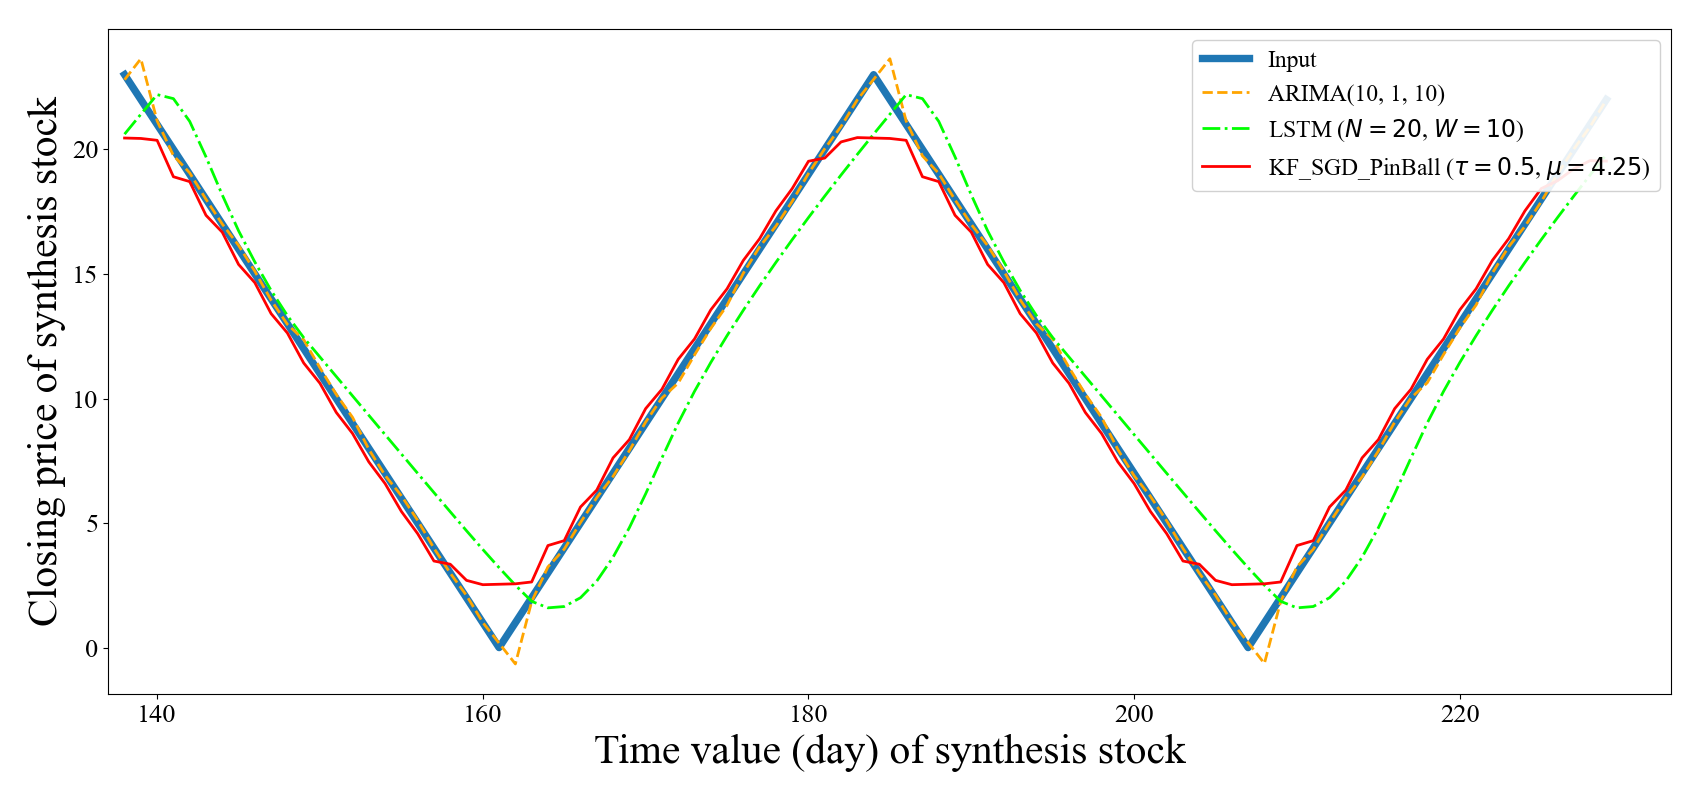
\includegraphics[width=\textwidth]{figure8a.png}
			\caption{The best Data-driven methods for prediction stock price.}
		\end{subfigure}
		\par\medskip
		\begin{subfigure}{0.8\textwidth}
			\centering
			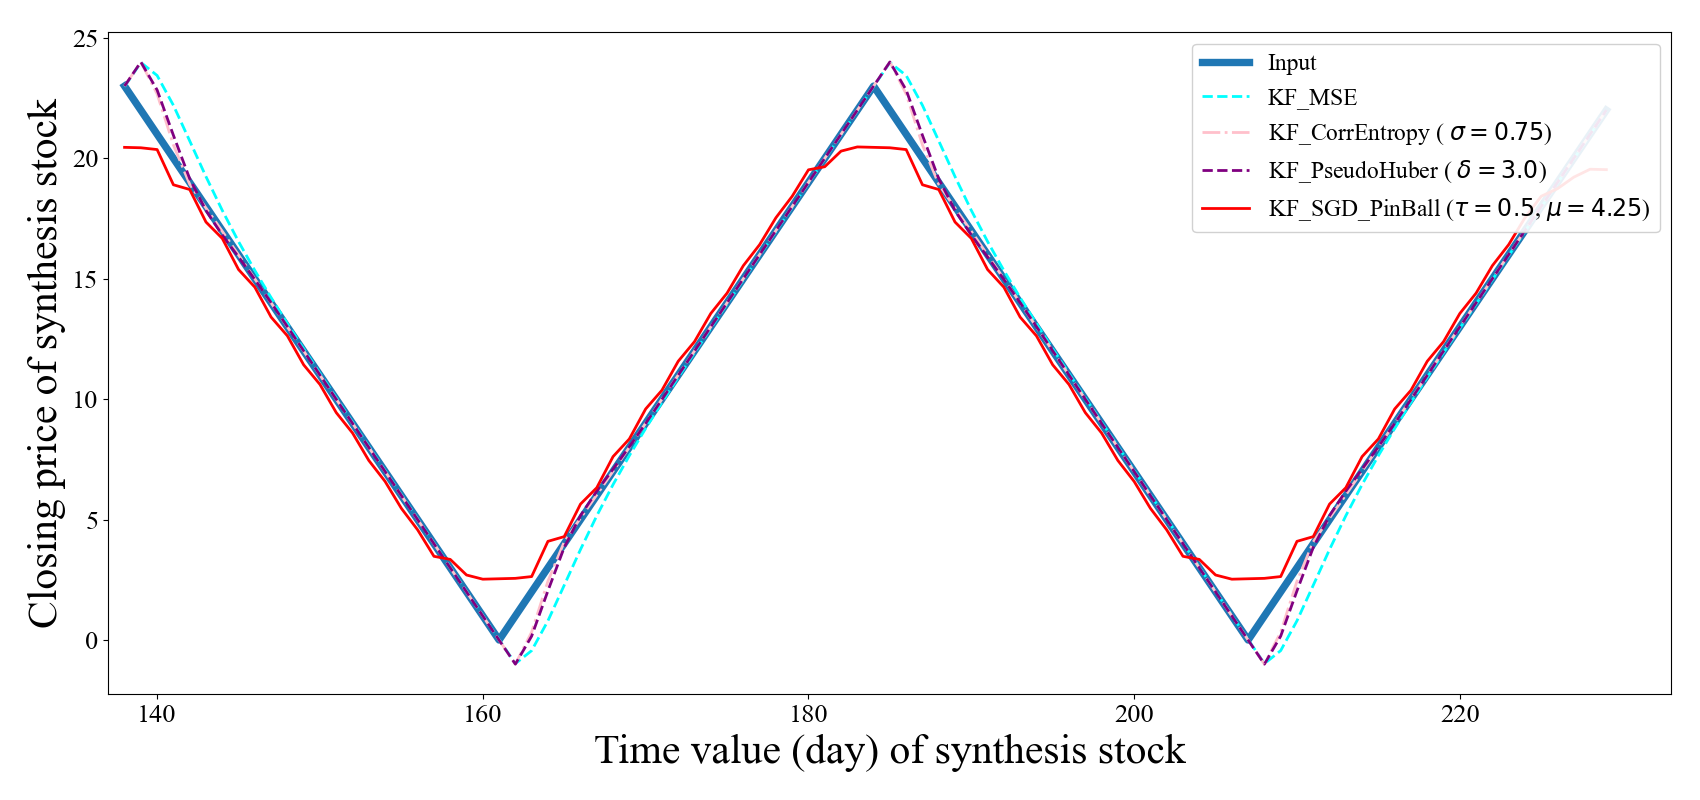
\includegraphics[width=\textwidth]{figure8b.png}
			\caption{The best Model-driven methods for prediction stock price.}
		\end{subfigure}
		\caption{The prediction of synthesis stock by data-driven and model-driven methods,both (a) and (b) illustrate that the controllable Kalman filter does better on reversal points with prior knowledge of those points.}
		\label{fig:figure8}
	\end{figure}
	
	\begin{figure}[H]
		\centering
		\begin{subfigure}{0.8\textwidth}
			\centering
			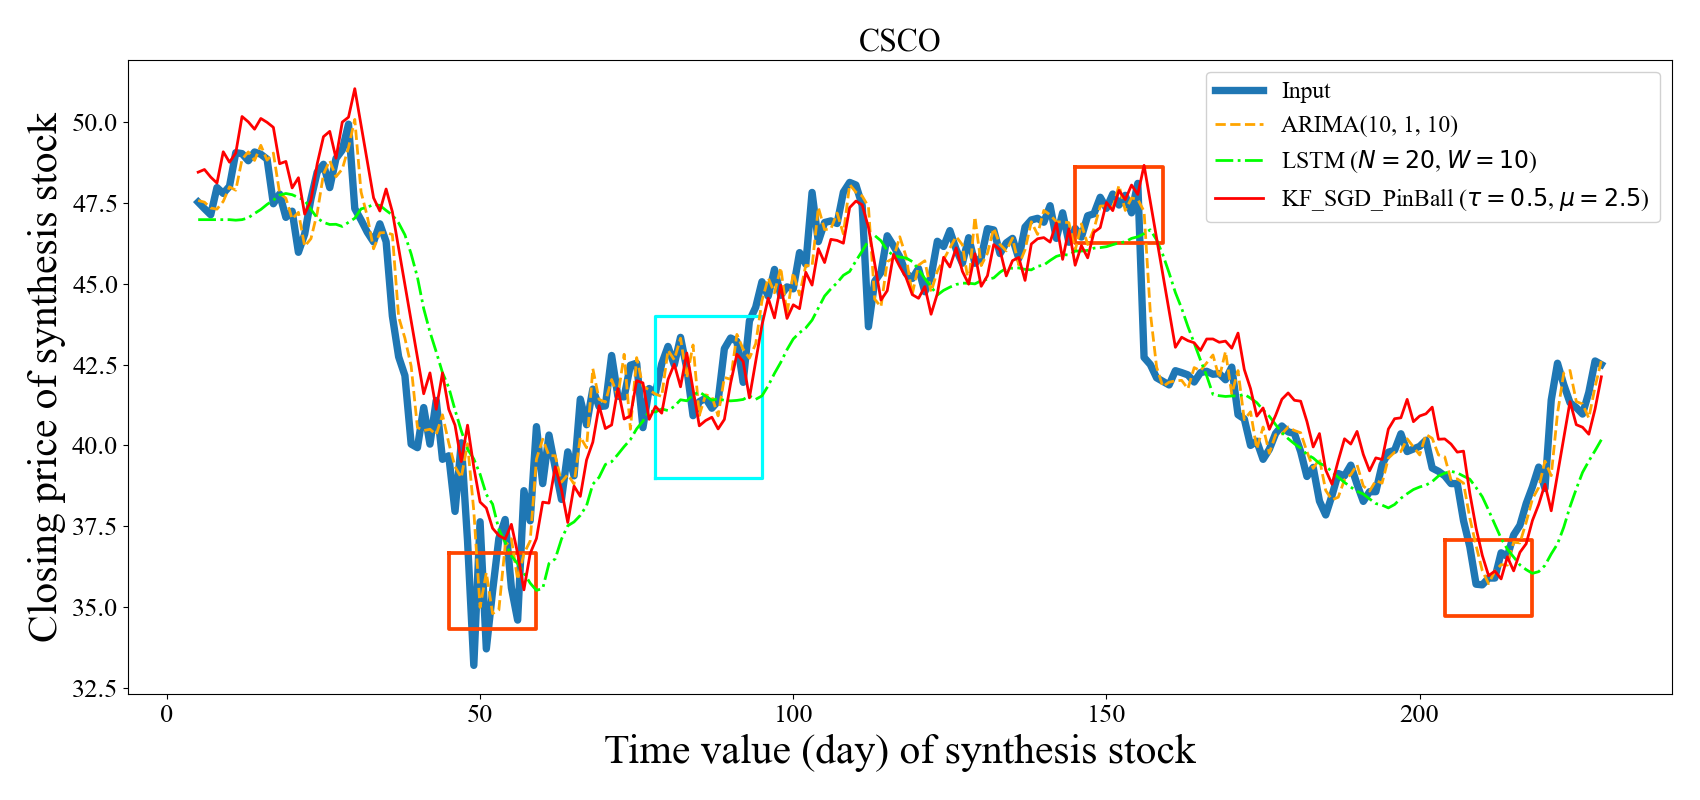
\includegraphics[width=\textwidth]{figure9a.png}
			\caption{The best Data-driven methods for prediction stock price.}
		\end{subfigure}
		\par\medskip
		\begin{subfigure}{0.8\textwidth}
			\centering
			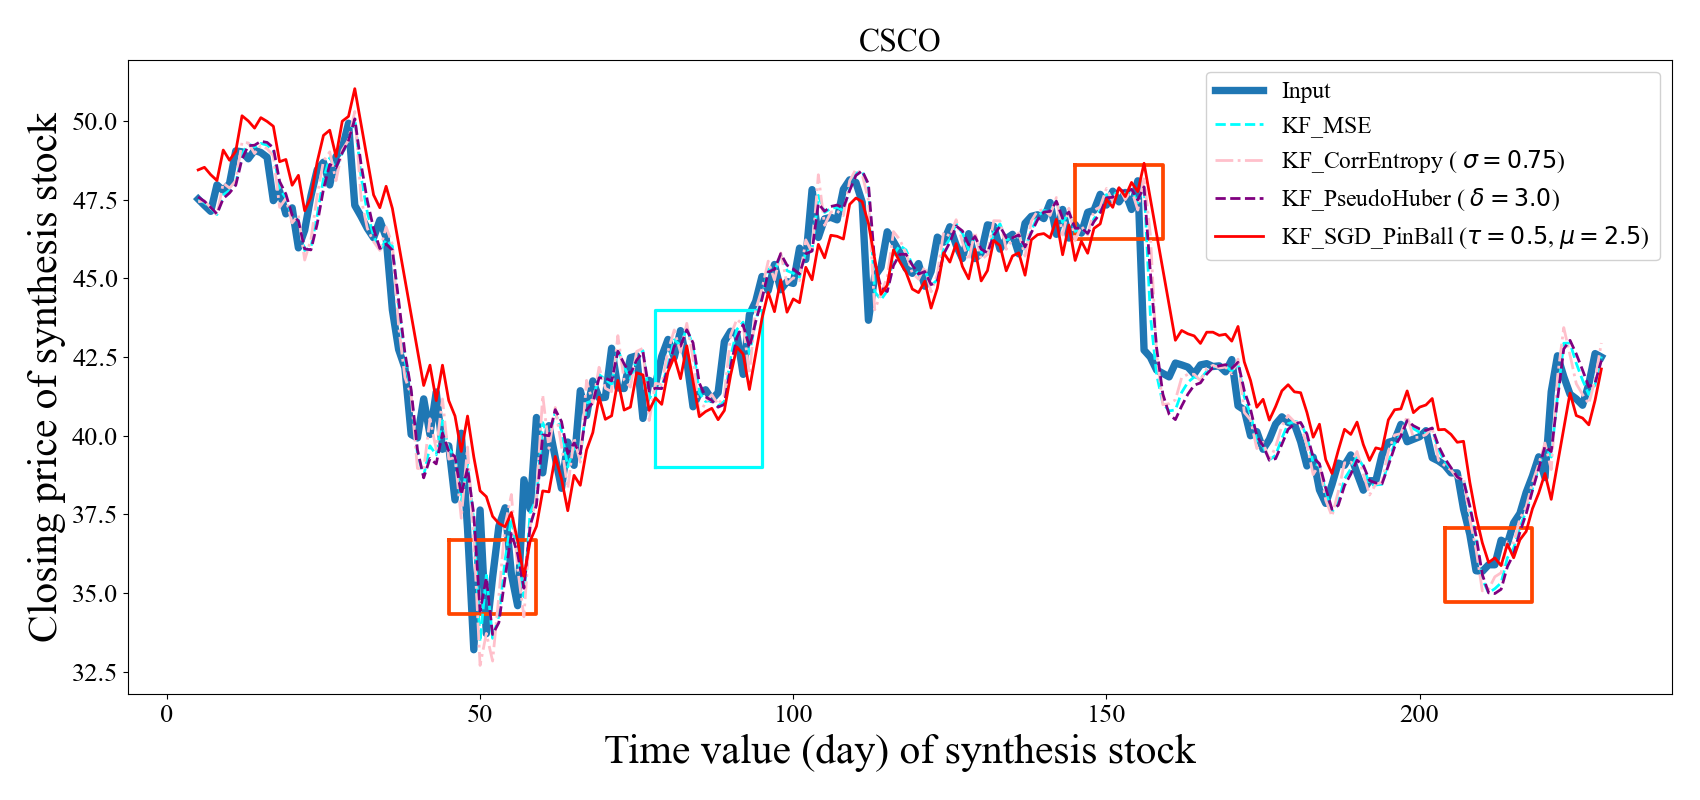
\includegraphics[width=\textwidth]{figure9b.png}
			\caption{The best Model-driven methods for prediction stock price.}
		\end{subfigure}
		\caption{The prediction of CSCO stock by data-driven and model-driven methods, the proposed method improves prediction at reversal points (red boxes) with the help of prior knowledge. Furthermore, without prior knowledge (cyan box), the proposed method does almost the same as other methods at other points that have a delay.}
		\label{fig:figure9}
	\end{figure}
	
	\subsection{Discussion}
	
	According to section 4.1, the objectives of this study are to analyze the effectiveness of the KF SGD Pinball algorithm at critical points. The aim is achieved by analyzing the profitability of stocks at critical points as well as by examining the loss functions of different stocks.
	
	In relation to the first research objective, the experiments gave the following conclusions:
	
	\begin{enumerate}
		\item Two methods based on the Kalman filter are introduced: KF Pseudo-Pinball and KF SGD pinball. KF SGD Pinball, for most stocks, comes out more profitable than both data-driven and model-driven methods. The result is compared with the best results from data-driven and model-driven approaches in the exact same structure. KF Pseudo-Pinball has better profit in peaks of GOOGL and the cause of introducing this approach and reporting its result is to analyze and interpret more on the Pinball loss function. The KF SGD Pinball method has the advantage of including more profit in the peaks and valleys of stock table 1.
	\end{enumerate}
	
	According to our experiments, the KF SGD Pinball algorithm in CISCO stock has less error in various loss functions than other algorithms. This point illustrates that this algorithm converges more rapidly after critical points than other methods. As a result of the second research objective, the following results were obtained:
	
	In terms of the experimental results of the second research objective, the benefit of the KF SGD Pinball algorithm is derived from its early return and early bypassing of the peaks. In addition, this algorithm bypasses valleys higher than the real valleys, and this early return is thought to be associated with profitability. According to the experiments of the second research goal, which is to determine the types of loss functions, the convergence of the KF SGD Pinball after passing through critical points is faster than other methods, which reduces the delay associated with returning from critical points.
	
	\section{Conclusion}
	
	This research proposes a new pinball loss function using Kalman filtering for stock price prediction. This function is non-derivative, so KF Pseudo-Pinball and KF SGD Pinball are defined. Pinball loss function behavior is controlled by prior knowledge during stock trading. An algorithm is utilized to extract prior knowledge, then apply it to the state space of the Kalman filter and adjust the Pinball loss function.
	
	We obtained experimental results from time series forecasting by experimenting with different stocks available on Yahoo Finance. On profit metrics in peaks and valleys as well as loss functions, we have shown how our model and other model-driven and data-driven models perform. According to our results, our modified Kalman filter performs better on most stocks.
	
	\sloppy
	\bibliographystyle{plain}
	\begin{thebibliography}{99}
		
		\bibitem{1} K. Sharma, R. Bhalla, Stock market prediction techniques: A review paper, in: Second International Conference on Sustainable Technologies for Computational Intelligence, Springer, 2022, pp. 175-188.
		
		\bibitem{2} S. H. Kang, H.-G. Cho, S.-M. Yoon, Modeling sudden volatility changes: Evidence from Japanese and Korean stock markets, Physica A: Statistical Mechanics and its Applications 388 (17) (2009) 3543-3550.
		
		\bibitem{3} G. Welch, G. Bishop, et al., An introduction to the kalman filter (1995).
		
		\bibitem{4} R. Izanloo, S. A. Fakoorian, H. S. Yazdi, D. Simon, Kalman filtering based on the maximum correntropy criterion in the presence of non-gaussian noise, in: 2016 Annual Conference on Information Science and Systems (CISS), IEEE, 2016, pp. 500-505.
		
		\bibitem{5} C. D. Karlgaard, Nonlinear regression huber-kalman filtering and fixed-interval smoothing, Journal of guidance, control, and dynamics 38 (2) (2015) 322-330.
		
		\bibitem{6} L. Chang, B. Hu, G. Chang, A. Li, Huber-based novel robust unscented kalman filter, IET Science, Measurement \& Technology 6 (6) (2012) 502-509.
		
		\bibitem{7} R. Adhikari, R. K. Agrawal, An introductory study on time series modeling and forecasting, arXiv preprint arXiv:1302.6613 (2013).
		
		\bibitem{8} Y. Zuo, E. Kita, Stock price forecast using bayesian network, Expert Systems with Applications 39 (8) (2012) 6729-6737.
		
		\bibitem{9} M. Nabipour, P. Nayyeri, H. Jabani, A. Mosavi, E. Salwana, Deep learning for stock market prediction, Entropy 22 (8) (2020) 840.
		
		\bibitem{10} S. L. Scott, H. R. Varian, Predicting the present with bayesian structural time series, International Journal of Mathematical Modelling and Numerical Optimisation 5 (1-2) (2014) 4-23.
		
		\bibitem{11} J. Qiu, S. R. Jammalamadaka, N. Ning, Multivariate bayesian structural time series model, J. Mach. Learn. Res. 19 (1) (2018) 2744-2776.
		
		\bibitem{12} N. Ning, J. Qiu, The mbts package: Multivariate bayesian structural time series models in r, arXiv preprint arXiv:2106.14045 (2021).
		
		\bibitem{13} M. A. Majidi, C.-S. Hsieh, H. S. Yazdi, Kalman filter reinforced by least mean square for systems with unknown inputs, Circuits, Systems, and Signal Processing 37 (11) (2018) 4955-4972.
		
		\bibitem{14} X. Lei, Z. Zhang, Recursive weighted least squares estimation algorithm based on minimum model error principle, Defence Technology 17 (2) (2021) 545-558. doi:https://doi.org/10.1016/j.dt.2020.02.003. URL https://www.sciencedirect.com/science/article/pii/S2214914719302636
		
		\bibitem{15} S. E. Azam, E. Chatzi, C. Papadimitriou, A dual kalman filter approach for state estimation via output-only acceleration measurements, Mechanical systems and signal processing 60 (2015) 866-886.
		
		\bibitem{16} A. Waheed, Analysis of moving average convergence divergence (macd) as a tool of equity trading at the karachi stock exchange (2013).
		
		\bibitem{17} W. Jiang, Applications of deep learning in stock market prediction: recent progress, Expert Systems with Applications 184 (2021) 115537.
		
		\bibitem{18} E. Rady, H. Fawzy, A. M. A. Fattah, Time series forecasting using tree based methods, J. Stat. Appl. Probab 10 (2021) 229-244.
		
		\bibitem{19} O. E. Orsel, S. S. Yamada, Comparative study of machine learning models for stock price prediction, arXiv preprint arXiv:2202.03156 (2022).
		
		\bibitem{20} S. Azman, D. Pathmanathan, A. Thavaneswaran, Forecasting the volatility of cryptocurrencies in the presence of covid-19 with the state space model and kalman filter, Mathematics 10 (17) (2022) 3190.
		
		\bibitem{21} M. Ganaie, M. Tanveer, Robust general twin support vector machine with pinball loss function, in: Machine Learning for Intelligent Multimedia Analytics, Springer, 2021, pp. 103-125.
		
		\bibitem{22} M. Tanveer, T. Gupta, M. Shah, A. D. N. Initiative, Pinball loss twin support vector clustering, ACM Transactions on Multimedia Computing, Communications, and Applications (TOMM) 17 (2s) (2021) 1-23.
		
		\bibitem{23} L. Li, S. Dai, Z. Cao, J. Hong, S. Jiang, K. Yang, Using improved gradient-boosted decision tree algorithm based on kalman filter (gbdt-kf) in time series prediction, The Journal of Supercomputing 76 (9) (2020) 6887-6900.
		
		\bibitem{24} F. Farahi, H. S. Yazdi, Probabilistic kalman filter for moving object tracking, Signal Processing: Image Communication 82 (2020) 115751.
		
		\bibitem{25} F. Arroyo-Marioli, F. Bullano, S. Kucinskas, C. Rondón-Moreno, Tracking r of covid-19: A new real-time estimation using the kalman filter, PloS one 16 (1) (2021) e0244474.
		
		\bibitem{26} S. V. Vaseghi, Advanced digital signal processing and noise reduction, John Wiley \& Sons, 2008.
		
		\bibitem{27} G. T. Cinar, J. C. Principe, Hidden state estimation using the correntropy filter with fixed point update and adaptive kernel size, in: The 2012 International Joint Conference on Neural Networks (IJCNN), IEEE, 2012, pp. 1-6.
		
		\bibitem{28} P. Charbonnier, L. Blanc-Féraud, G. Aubert, M. Barlaud, Deterministic edge-preserving regularization in computed imaging, IEEE Transactions on image processing 6 (2) (1997) 298-311.
		
		\bibitem{29} K. Kohara, T. Ishikawa, Y. Fukuhara, Y. Nakamura, Stock price prediction using prior knowledge and neural networks, Intelligent Systems in Accounting, Finance \& Management 6 (1) (1997) 11-22.
		
		\bibitem{30} K. Dhanasekaren, S. T. Aluri, N. Karthikeyan, S. H. Baskaran, R. Selvanambi, A study on the impact of sentiment analysis on stock market prediction, Recent Advances in Computer Science and Communications (Formerly: Recent Patents on Computer Science) 16 (1) (2023) 73-93.
		
		\bibitem{31} H. Masnadi-Shirazi, A. Masnadi-Shirazi, M.-A. Dastgheib, A step by step mathematical derivation and tutorial on kalman filters, arXiv preprint arXiv:1910.03558 (2019).
		
	\end{thebibliography}
	
\end{document}
